\chapter{Konzepte \& Architektur}
\label{ch:konzepte_architektur}
\section{Konzepte}
Für die Bewältigung der Anforderungen an die Softwarelösung wurden einige Konzepte entwickelt, welche Einfluss auf die einzelnen Komponenten und die Architektur genommen haben. Die Softwarelösung soll wie unter \ref{ch:anforderungen_section} \nameref{ch:anforderungen_section} beschrieben, die Möglichkeit bieten eine Karte darzustellen, auf welcher die Simulationsdaten dargestellt werden und bearbeitet werden können. Die Bearbeitung sollte jedoch keinen Einfluss auf die Stammdaten haben. Diese Konzepte werden in den folgenden Kapiteln beschrieben.\\
\textbf{\textit{TODO}}
Um die Anforderungen (siehe. \ref{ch:anforderungen_section}) an die Softwarelösung zu bewältigen, wurden Konzepte für die einzelnen Komponenten entwickelt, welche Einfluss auf die Architektur haben.
\subsection{Datentiles}
\label{ch:datentiles}
Um die grosse Datenmenge (ca. 2,8 Millionen Datensätze für die Schweiz) zu bewältigen, wurde ein bewährtes Verfahren für Kartendarstellung verwendet. Dabei werden die Daten nicht als gesamtes geliefert, sondern über Tiles angefragt. Ein Tile ist ein Quadrat, welches ein vordefinierten Bereich der Welt deckt. Durch die Anforderung eines dieser Quadrate kann sichergestellt werden, dass nicht zu viele Daten auf einmal angefragt werden. Ein weiteres Konzept in Verbindung mit diesem wird unter \ref{sec:concept_preprocessing} \nameref{sec:concept_preprocessing} beschrieben. Dabei werden die Daten für jede Zoomstufe bewertet und nur ausgegeben, wenn diese Relevant sind. Durch dieses Konzept kann die Datenmenge, die von der Website verarbeitet werden muss, stark reduziert werden.
\begin{figure}[H]
\centering
\includegraphics[height=7cm]{images/BingMapsTileSystem.jpg}
\\Quelle: \href{https://msdn.microsoft.com/en-us/library/bb259689.aspx}{https://msdn.microsoft.com/en-us/library/bb259689.aspx}
\caption{Fixe Aufteilung der Welt in Tiles und Berechnung des QuadKey}
\label{fig:tilesystem}
\end{figure}
\noindent
Um von einem Eintrag auf das Tile zu schliessen, in welchem dieser sichtbar ist, wird ein Schlüssel (QuadKey) berechnet. Der QuadKey benennt eindeutig das kleinstmögliche Tile in welchem der ganze Eintrag (z.B. eine Strasse) angezeigt werden kann. Der QuadKey wird nach dem System in Abbildung \ref{fig:tilesystem} erstellt. Dabei wird auf der äussersten Zoomstufe die Welt in 4 Tiles aufgeteilt. Diese werden nummeriert. z.B. 0 für links oben, 1 für rechts oben. Um die nächste Stufe der Tiles zu erstellen, wird jedes Tile wieder in 4 Tiles aufgeteilt und dann ebenfalls nummeriert. Dabei wird als Prefix die Nummer des alten Tiles verwendet. Dadurch kann jedes Tile auf jeder Zoomstufe eindeutig adressiert werden. Der QuadKey bietet auch die Möglichkeit, mit Hilfe des Prefix alle Tiles unterhalb eines Tiles zu berechnen. So starten alle QuadKeys, welche auf einer beliebigen Zoomstufe in einem Tile unterhalb des linken oberen Tile auf Level 1 sind, mit einer 0. Dieser Ansatz kann für die Filterung der Daten verwendet werden.
\subsection{Preprocessing und Bewertung der Daten}\label{sec:concept_preprocessing}
Um die Zugriffszeiten der Datenbank zu erhöhen, werden die Daten beim Importieren vorberechnet. Durch diesen Vorgang werden bewusst Redundanzen in das Datenmodell eingeführt. Diese Redundanzen erlauben den Zugriff auf Daten ohne teure JOIN Statements oder SQL-Funktionen aufzurufen. Auf die Vorberechnungen, welche im Datenmodell verwendet werden, wird tiefer im Abschnitt \ref{sec:tilingdataimplementation} \nameref{sec:tilingdataimplementation} eingegangen. Um weiteren Berechnungsaufwand zu reduzieren, wird jeder Datensatz neben der Vorberechnung auf seine Anzeigewichtigkeit bewertet. Dabei wird berechnet, ab welcher Stufe z.B. die Strasse dargestellt wird.

\subsection{Changeset}\label{sec:changeset}
Um Daten der User abzuspeichern wurde ein Konzept entwickelt, mit welchem erreicht werden soll, dass Daten gespeichert werden können ohne die Stammdaten anzupassen. Wenn für jeden User die Stammdaten kopiert werden müssten, würde das zu einer unnötigen Vergrösserung der Datenmenge führen. Dadurch wurde das Changeset Konzept entwickelt. Changesets erlauben es, Änderungen aufzuteilen und nur die Differenz zu den Stammdaten abzulegen. Dadurch wird es ermöglicht die Zugriffszeiten auf die Stammdaten konstant zu halten. Das Changeset ist als Abbild der Stammdaten aufgebaut. Dabei werden jedoch nur Felder gespeichert, welche sich zu den Stammdaten unterscheiden. Da ein Changeset nicht direkt Stammdaten enthält werden Änderungen an den Stammdaten übernommen, so fern sie nicht durch das Changeset bearbeitet wurden.
\subsection{UI-Konzept}\label{sec:uiconcept}
Das UI ist eine zentrale Komponente des Verkehrsmodell-Fallstudien-Editor. Daher muss ein einfaches und intuitives Konzept entwickelt werden, welches wenig Einarbeitungszeit braucht. Als Inspirationsquelle für das User Handling wurde Google Maps \cite{GoogleMaps}, sowie der ID Editor \citep{IDEditor} von OpenStreetMap verwendet, da sie zwei weit verbreitete und oft genutzte Anwendungen sind, welche ein durchdachtes Design besitzen.\\[0.8cm]
\textbf{evtl. TODO Hauptaufgaben des UI Darstellen (evtl mit Grafik)}
\newpage
\subsubsection{Google Maps}
Google Maps ist eines der weit verbreitetsten Kartensysteme. Dadurch sind sich die User an das Handling von Google Maps gewöhnt und Systeme mit ähnlichen Aufbau sind intuitiv. Die Vorteile des System von Google Map ist die intuitive Bedienung, gekoppelt an ein einfaches, aufgeräumtes und leichten Design.
\begin{figure}[H]
\centering
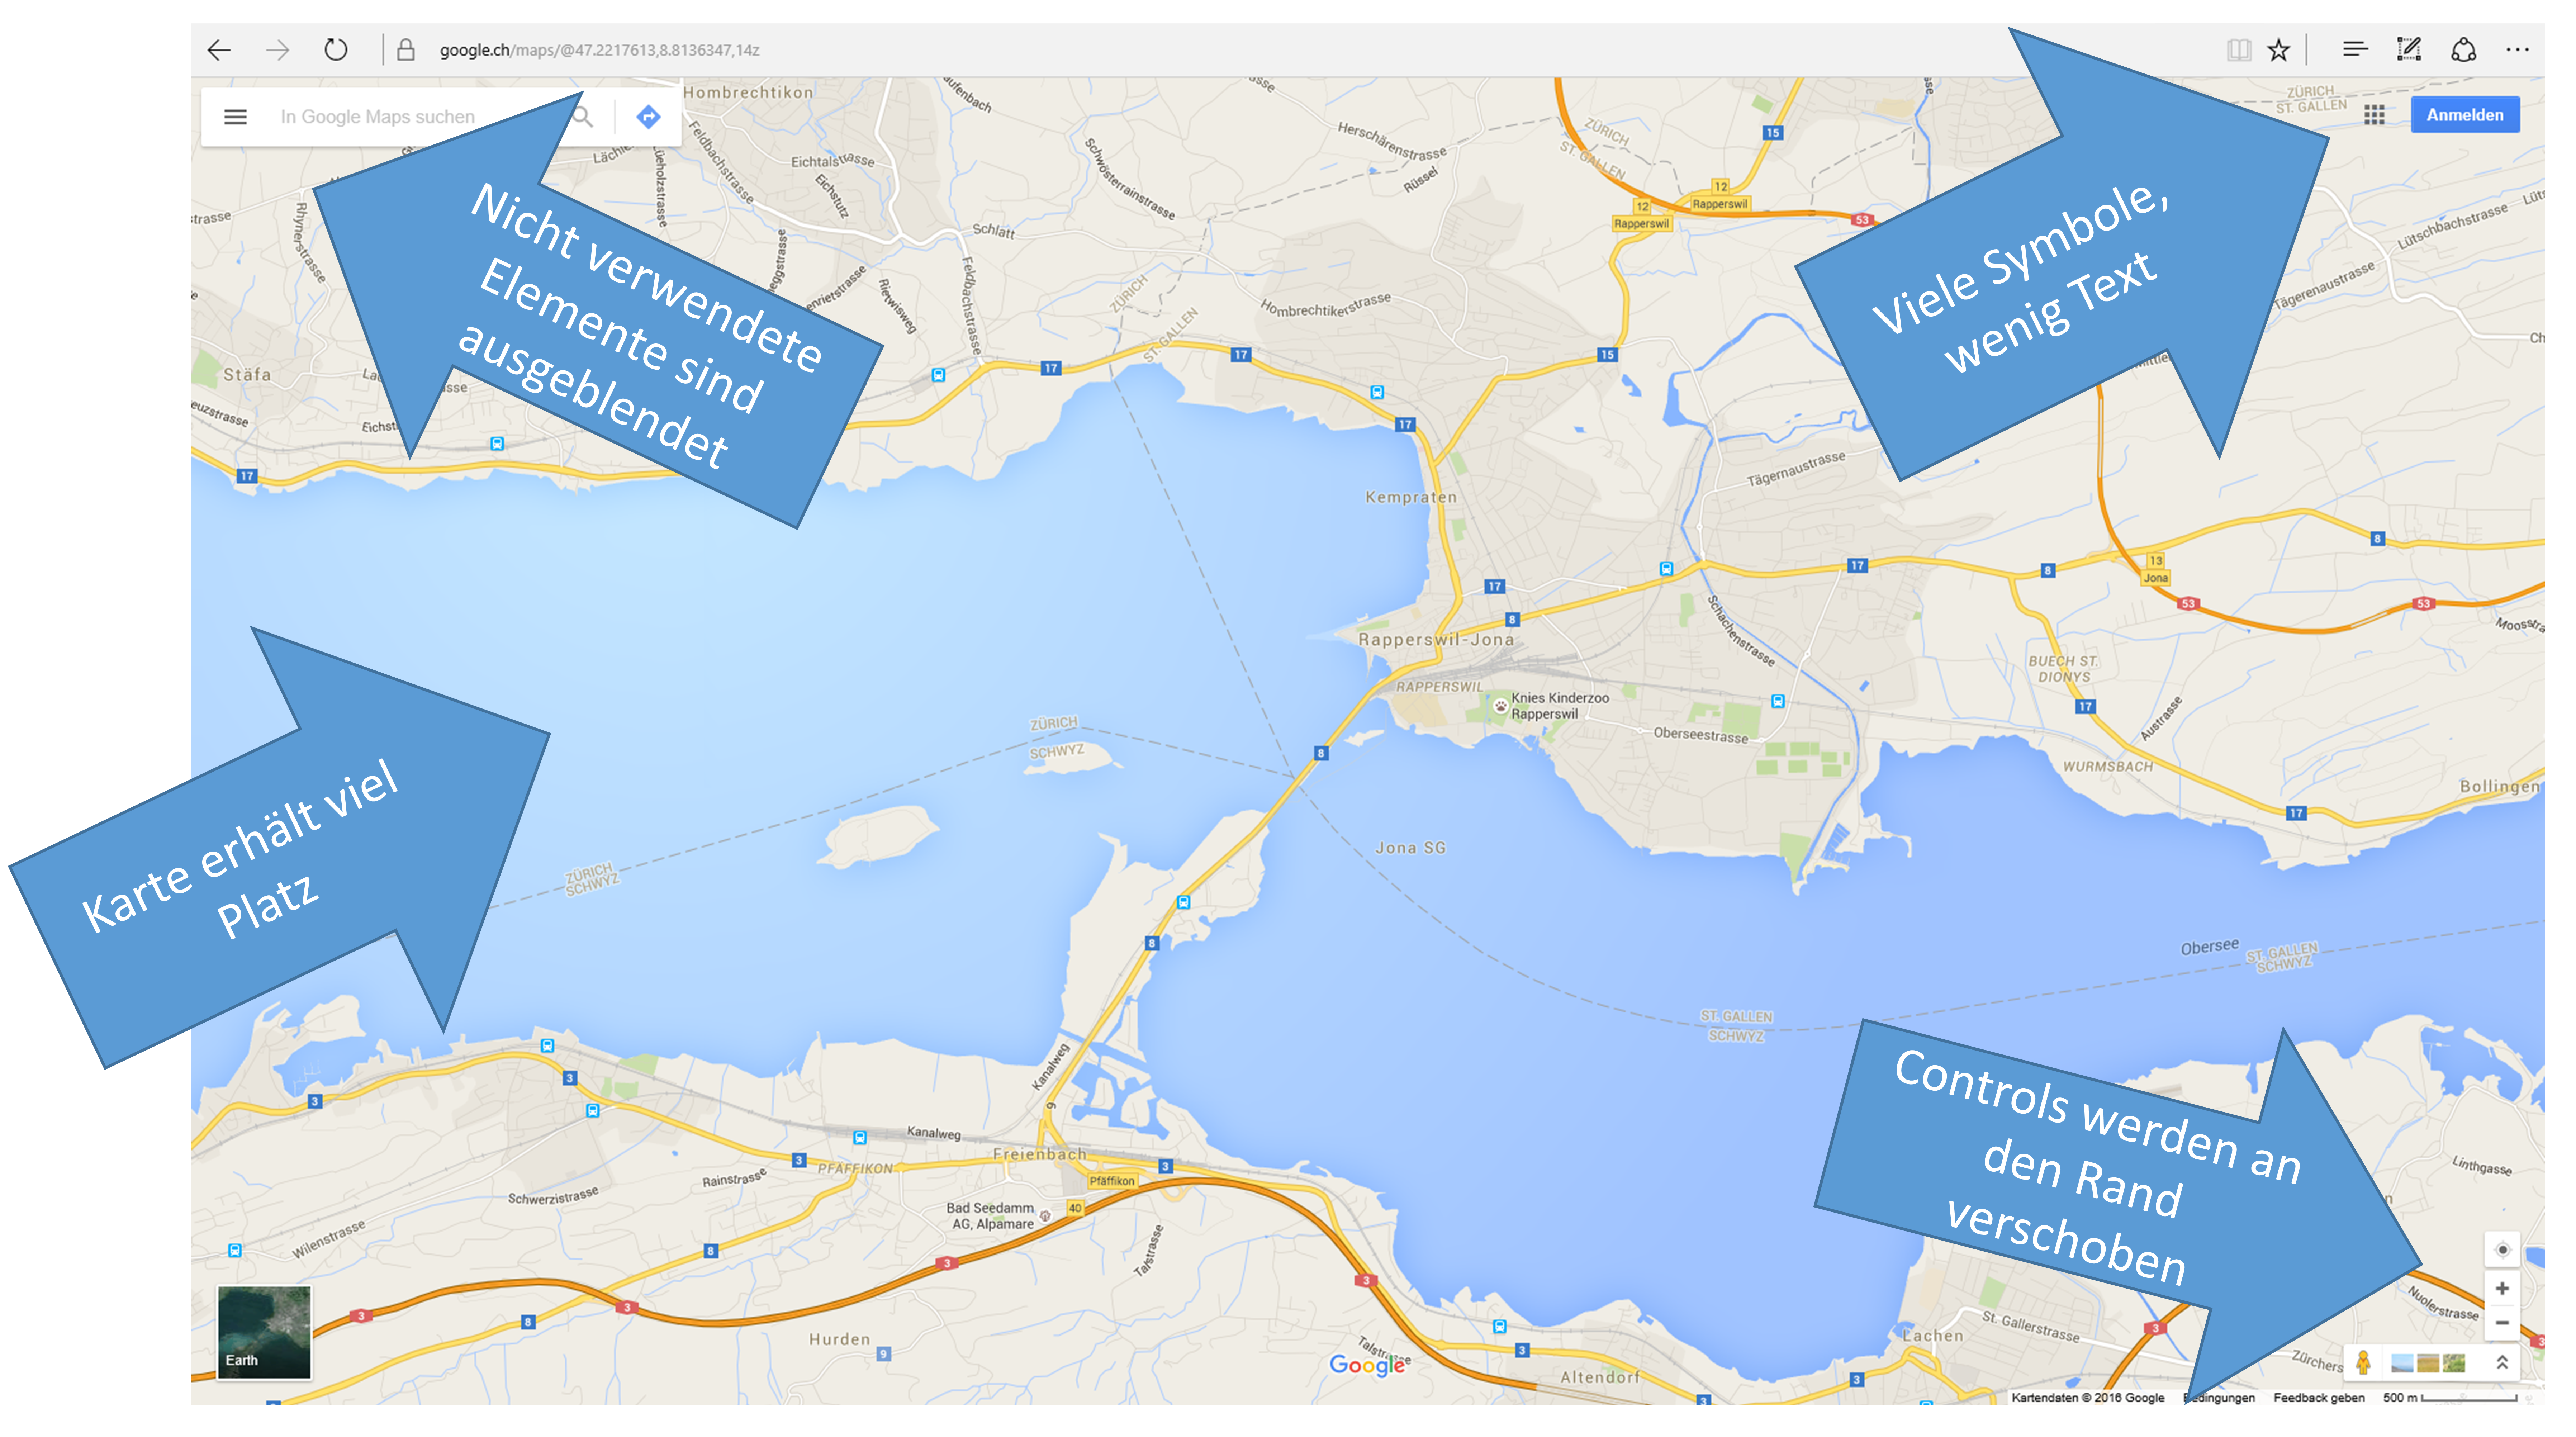
\includegraphics[height=7cm]{images/AnalyseGoogle.png}
\caption{Analyse Google Maps}
\label{fig:googlemaps}
\end{figure}
\noindent
Die Abbildung \ref{fig:googlemaps} \nameref{fig:googlemaps} zeigt die Analyse von Google Maps. Die Karte bei Google Maps erhält sehr viel Platz und alle Controls werden um den Hauptbereich der Karte herum angeordnet. Dadurch wird der User nicht von der Kernaufgabe der Seite abgelenkt. Bei kleineren Karten fühlt sich der User schneller eingegrenzt muss mehr aufwand in Scrolling investieren, was stören kann. Das User Interface passt sich laufend an die Nutzung des Users an. Wenn der User also fertig ist, ein Ort zu finden und eine Route berechnen will, wird das Menü für die Route seitlich eingeblendet. Dadurch wird der Karte Platz weggenommen, welcher jedoch nicht mehr benötigt wird, da der User eine Route berechnen will. Um Platz für die Controls zu sparen, werden viele Symbole anstatt Text eingesetzt.
\subsubsection*{Ergebnisse Analyse}
Die Analyse von Google Maps ergab folgende Punkte, welche in das Design des Verkehrsmodell-Fallstudien-Editors einfliessen sollen:
\begin{itemize}
\item Der Karte viel Platz einräumen.
\item Menüs, welche nicht dem aktuellen Use Case entsprechen, ausblenden.
\item Viele Symbole, wenig Text.
\end{itemize}
\newpage
\subsubsection{ID Editor}
Der ID Editor von OpenStreetMap ist der bekannteste Editor für OpenStreetMap. Er bietet die Möglichkeit Daten von OpenStreetMap direkt auf einer Karte zu bearbeiten. Die Änderungen werden dann als Changeset an OpenStreetMap übertragen und freigeschaltet. Da die Funktionen des ID Editor sehr ähnlich wie die Funktionen des Verkehrsmodell-Fallstudien Editor sind, wurde das UI des ID Editor ebenfalls analysiert.
\begin{figure}[H]
\centering
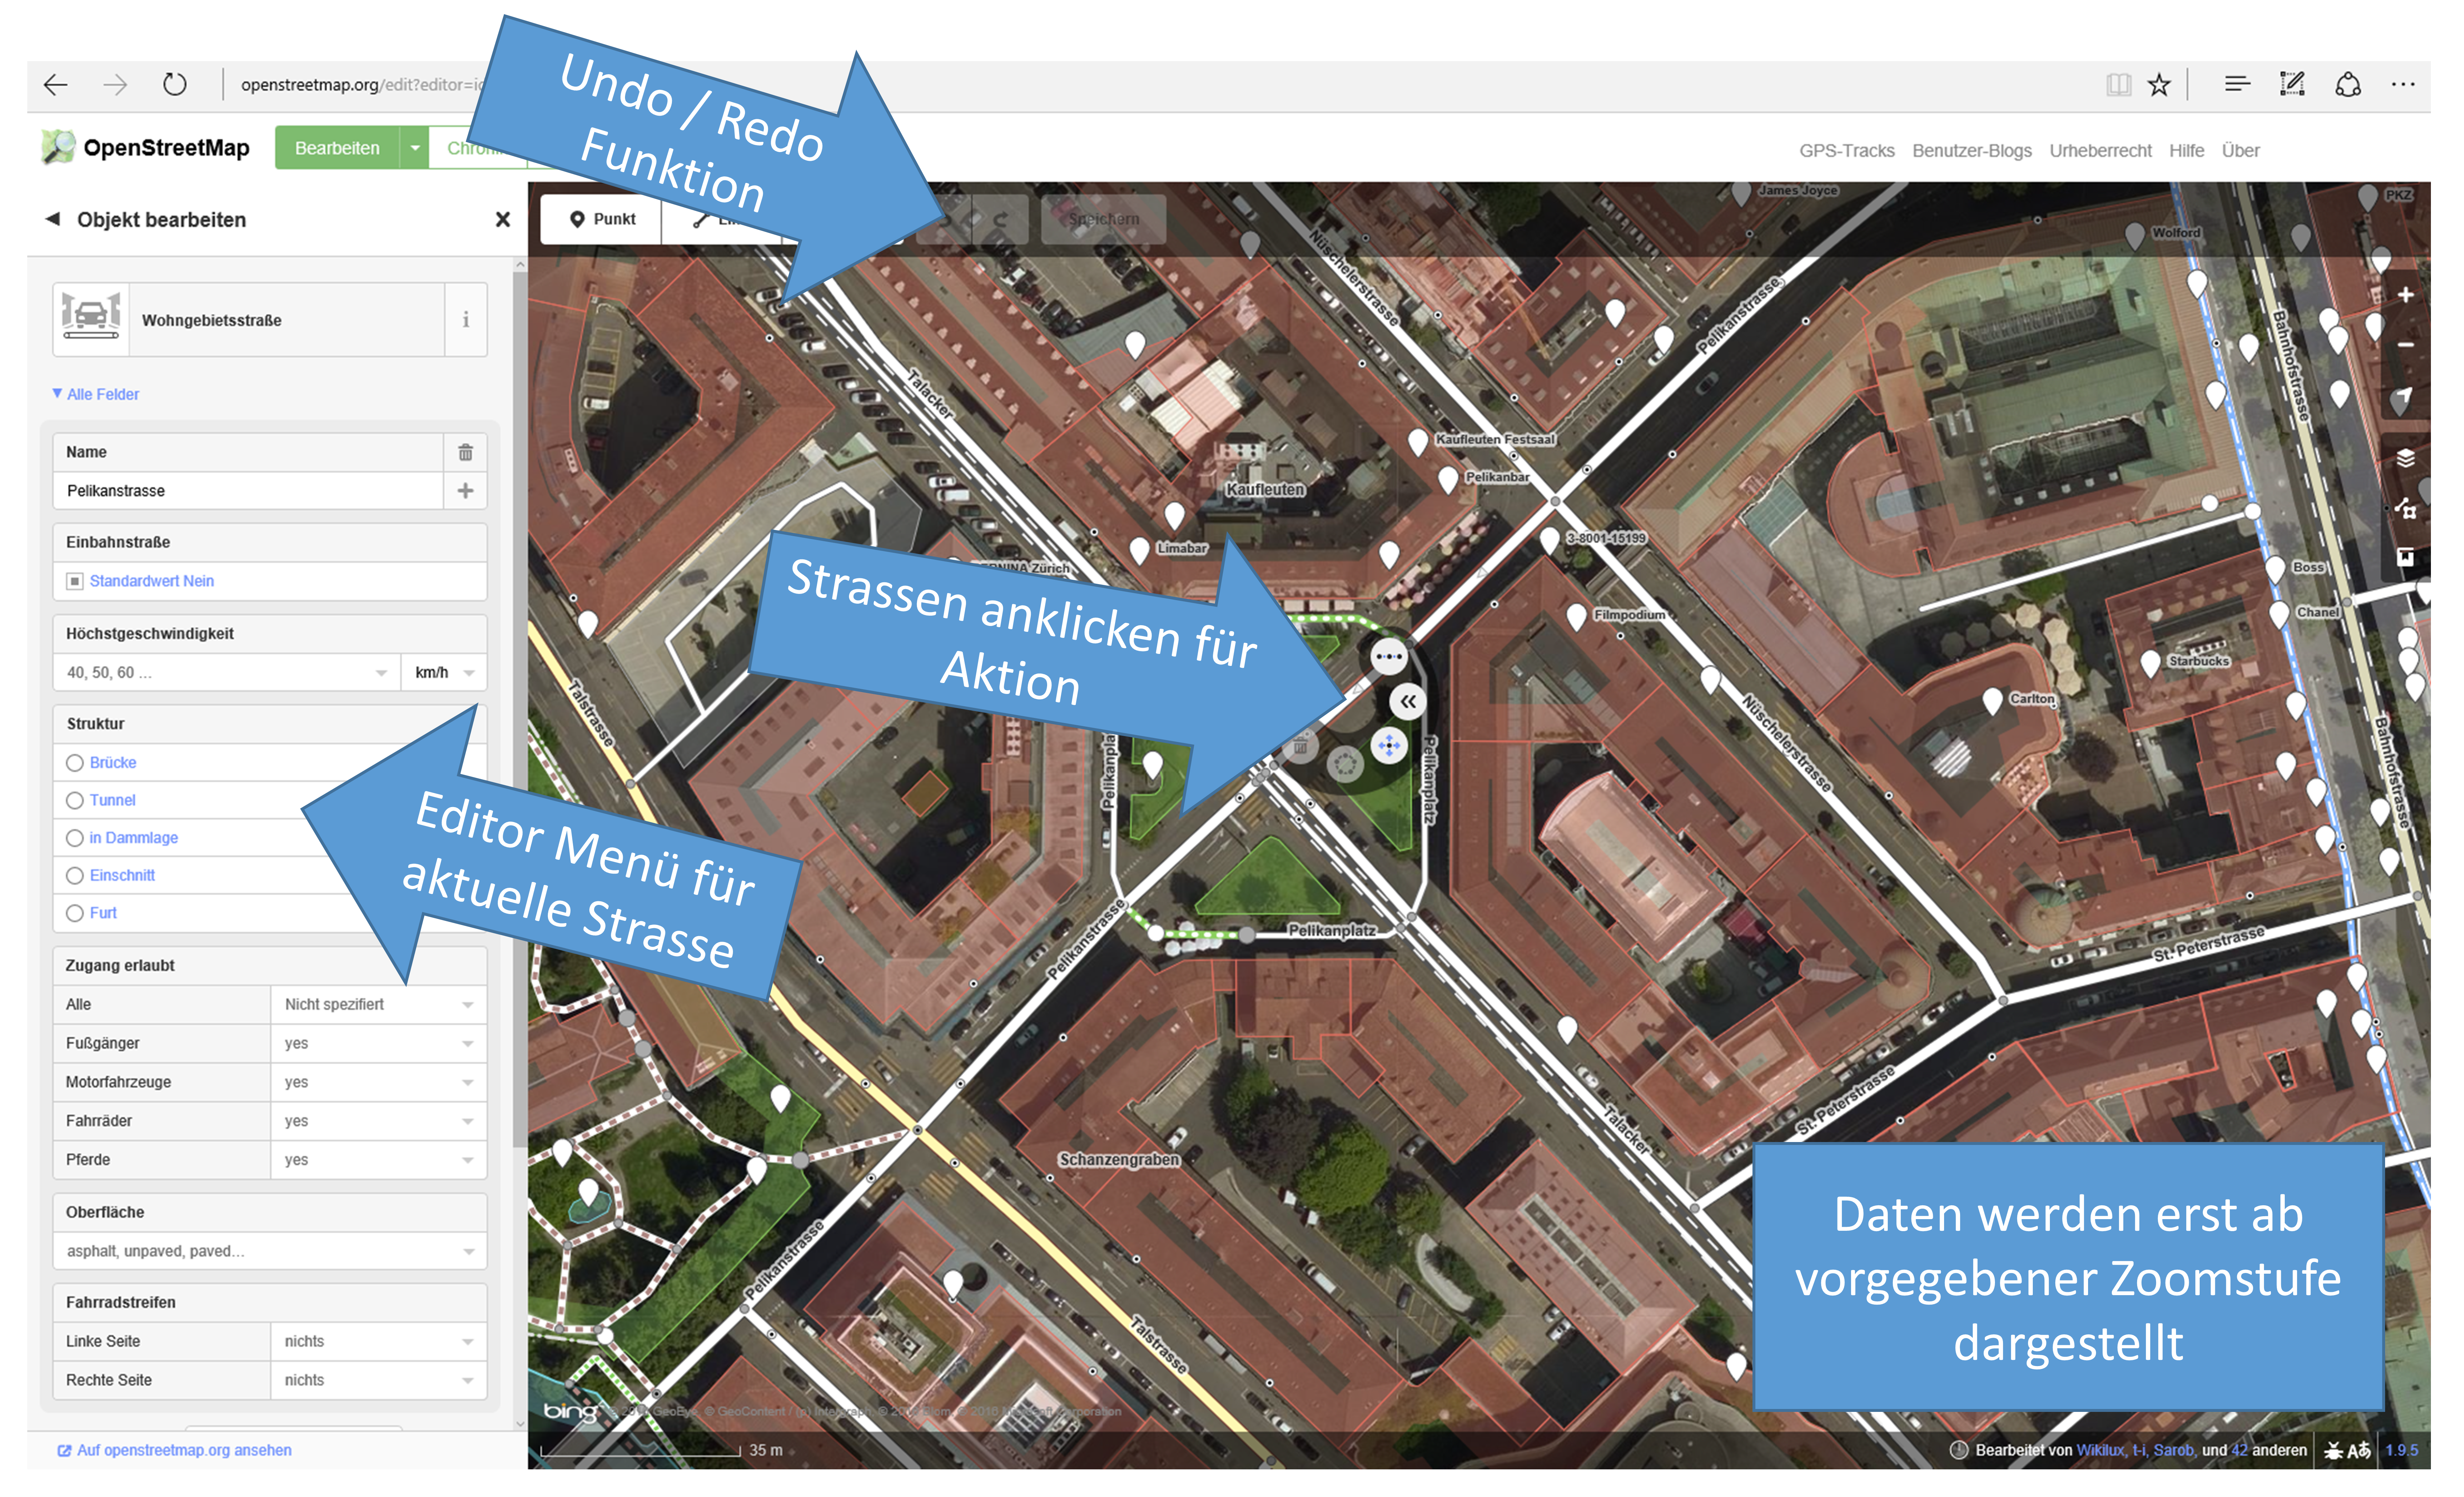
\includegraphics[height=7cm]{images/AnalyseIDEditor.png}
\caption{Analyse ID Editor}
\label{fig:ideditor}
\end{figure}
\noindent
In der Abbildung \ref{fig:ideditor} \nameref{fig:ideditor} wird die Analyse des ID Editor gezeigt. Um die Datenmenge, welche OpenStreetMap für die Kartenerstellung braucht, verwalten zu können, ist ein wichtiges Element des User Interface, dass die Daten erst dargestellt werden, wenn der User nahe genug herangezoomed hat. Dies ermöglicht es dem ID Editor die Datenmenge, welche zur selben Zeit dargestellt werden soll, auf ein Minimum zu reduzieren. Das Editormenü des ID Editor ist so aufgebaut, dass eine Strasse angeklickt wird und die Strasse dann in einem Sidepanel dargestellt wird. Dabei wird die Karte nicht ausgeblendet, was eine leichte und schnelle Bedienung für den User ermöglicht. Weiter besitzt der ID Editor eine gute Undo- / Redofunktion. Änderungen welche an Objekten vorgenommen werden, können einfach wieder rückgängig gemacht werden.
\subsubsection*{Ergebnisse Analyse}
Für das Design-Konzept des Verkehrsmodell-Fallstudien-Editors ergeben sich folgende Punkte aus der Analyse:
\begin{itemize}
\item Kein Wechsel der Website zur Bearbeitung von Strassenattributen.
\item Strassen durch anklicken bearbeiten.
\item Undo- /Redofunktion.
\end{itemize}
\newpage
\subsubsection{Detail Konzept}
Aus den Erkenntnissen der Analyse von Google Maps und dem ID Editor wurde ein Konzept für das UI des Verkehrsmodell-Fallstudien Editor entwickelt.
\begin{figure}[H]
\centering
\includegraphics[height=7cm]{images/KonzeptUI.png}
\caption{Wireframe Editor}
\label{fig:conceptui}
\end{figure}
\noindent
Das Userinterface wird, angelehnt an Google Maps, eine Karte besitzen, welche den Browser ausfüllt. Menüs, welche nicht gebraucht werden, sind, wie in Abbildung \ref{fig:conceptui} \nameref{fig:conceptui} dargestellt, ausgeblendet. Dadurch hat der User viel Platz, die für ihn relevante Strasse zu suchen. Durch das Auswählen einer Strasse, wird ein Menü von der Seite eingeblendet, welches das Bearbeiten der Parameter dieser Strasse erlaubt. (sh. Abbildung \ref{fig:concepteditStreet} \nameref{fig:concepteditStreet}). Zudem bietet die Software eine Undo- / Redofunktion.
\begin{figure}[H]
\centering
\includegraphics[height=7cm]{images/KonzeptEditStreet.png}
\caption{Wireframe Strassenattribute bearbeiten}
\label{fig:concepteditStreet}
\end{figure}
\newpage
\noindent
Um die Wegführung einer Strasse zu bearbeiten kann der User in einen Bearbeitungsmodus wechseln. In dem er dann eine Strasse anklicken kann und die Führung der Strasse in einem Menü verändern. Die dafür benötigten Nodes, werden aus Performancegründen nur im Bearbeitungsmodus geladen und angezeigt.
\begin{figure}[H]
\centering
\includegraphics[height=7cm]{images/KonzeptChangeStreet.PNG}
\caption{Wireframe Strassenführung bearbeiten}
\label{fig:concepteditStreet}
\end{figure}
\noindent
Ein weiteres, naheliegendes Konzept für die Bearbeitung der Strassenführung, wäre ein Drag \& Drop Verfahren. Dieses Konzept wäre für den Benutzer am einfachsten, ist jedoch sehr zeitintensiv in der Implementation. Aus Zeitgründen musste dadurch auf Drag \& Drop verzichtet werden.
\section{Architektur}
\begin{figure}[H]
\centering
\includegraphics[height=10cm]{images/Architektur.png}
\caption{Tier des Verkehrsmodell-Fallstudien-Editor}
\label{tier_architecture}
\end{figure}
Durch die Anforderungen bezüglich Performance und Antwortgeschwindigkeiten musste die Architektur für die Softwarelösung des Verkehrsmodell-Fallstudien-Editor skalierbar aufgebaut werden. Eine Entkopplung der Komponenten erlaubt eine Verteilung und kann daher die Last auf dem einzelnen Server senken. Die Softwarelösung für den Verkehrsmodell-Fallstudien-Editor ist daher als 3-Tier Applikation aufgebaut. Der Frontside-Tier ist ein Webprojekt implementiert mit dem Play Framework. Der Backend-Tier wird als REST Service (Maturity Level 2) mit Dropwizard entwickelt. Der Daten-Tier wird durch eine PostgreSQL Datenbank bereitgestellt. Der Backend-Tier wird durch eine Load Balancer skalierbar und kann daher mehrere Anfragen parallel ausführen.\\
\begin{figure}[H]
\centering
\includegraphics[height=10cm]{images/layers.png}
\caption{Tier- / Layeraufteilung}
\label{fig:tierlayers}
\end{figure}
\noindent
Die Aufteilung der Presentation Logic auf den Client-Tier, sowie den Backend-Tier erlaubt es die Last der Datendarstellung auf die verschiedenen Komponenten zu verteilen. Die Vorbereitung und Aufbereitung der Daten wird vom Backend-Tier vorgenommen. Die Daten werden im für den Client lesbaren Format übertragen. Das Rendering der Daten übernimmt dann der Client, was dazu führt, dass der Server bei diesen Aufgaben entlastet wird.
\newpage
\section{SimMapEditor}
\begin{figure}[H]
\centering
\includegraphics[height=2cm]{images/presentationlayer.png}
\caption{SimMapEditor}
\label{fig:presentationlayer}
\end{figure}
\noindent
Der SimMap-Editor ist die Frontend-Komponente der Architektur und basiert auf dem Play Framework. Der Client Tier ist eine in Javascript entwickelte Software, welche auf den Backend-Tier zugreift, um die Daten auf der Karte darzustellen. Dabei übernimmt der Client-Tier das Rendering der Daten.
Der SimMapEditor ist die Frontend-Komponente der Achitektur. Der Client Tier wird in Javascript entwickelt und wird als Play Framework Projekt erstellt. Der Client Tier besitzt jedoch keine eigene Business Logic. Diese wird auf den Backend Tier ausgelagert und ist daher nicht im Play Framework implementiert. Der Client Tier ist dafür zuständig das UI Konzept (sh. \ref{sec:uiconcept} \nameref{sec:uiconcept}) zu implementieren und die Daten für die Karte vom Backend Tier anzufordern. Dazu muss der Client Tier das Tilesystem (sh. \ref{ch:datentiles} \nameref{ch:datentiles} ) implementieren und die Daten nach Tiles vom Backend Tier abfragen.
\section{SimMapService}
\begin{figure}[H]
\centering
\includegraphics[height=5.5cm]{images/BusinessLogicLayer.png}
\caption{SimMapService}
\label{fig:businesslogiclayer}
\end{figure}
\noindent
Der SimMapService implementiert den Backend Tier der Softwarelösung in einer 3 Layer Architektur. Er wird als REST Service (Maturity Level 2 \cite{RESTMaturity} ) entwickelt. Um dem Maturity Level 2 zu entsprechen, werden die Anfragen und Antworten des Services mit HTTP Standard Methoden und Codes ausgestattet. Mit den Codes wird dem Client angezeigt, welchen Status die Antwort hat. Z.B. Wird bei einer erfolgreichen Abfrage, welche keine Daten zurückgibt, der Code 201 No Content zurückgesendet. Dies zeigt dem Client, dass er keine Daten erwarten soll, sondern vorgesehen ist das der Body der Antwort leer ist. Für den Aufbau der Antworten mit den korrekten Codes und Umwandlung der Objekte in JSON ist der Presentation Logic Layer des SimMapService zuständig.\\
Der Application Logic Layer des SimMapService ist dafür zuständig die Daten zusammenzufügen und die Preprocessings, welche im Kapitel \ref{sec:concept_preprocessing} \nameref{sec:concept_preprocessing} beschrieben sind, durchzuführen. Er lädt Daten aus dem Resource Layer je nach Zoomlevel und Koordinaten, bereitet dann die Daten auf und übergibt sie dem Presentation Logic Layer.\\
Der Resource Logic Layer bietet dem Application Logic Layer alle Methoden, welche für den Datenzugriff genutzt werden müssen. Seine Aufgabe ist die Erstellung und Durchführung der Abfragen auf die Datenbank.
\section{Datenbank}
\begin{figure}[H]
\centering
\includegraphics[height=2cm]{images/Database.png}
\caption{Datenbank}
\label{fig:database}
\end{figure}
\noindent
Wegen der grossen Datenmenge welche mit der Softwarelösung des Verkehrsmodell-Fallstudien-Editor verwaltet werden soll, ist die Datenbank ein essenzieller Teil der Architektur. Das Datenmodell wurde darauf ausgelegt die Datenmenge der Stammdaten, von den Daten der Changesets (sh. \ref{sec:changeset} \nameref{sec:changeset}) zu trennen. Dadurch wird die Zugriffszeit auf die Stammdaten nicht durch die Datenmenge der User beeinflusst, sondern bleibt unabhängig.
\begin{figure}[H]
\centering
\includegraphics[height=10cm]{images/SimmapDatabase.jpg}
\caption{ERP der Datenbank}
\label{fig:databasescheme}
\end{figure}
\noindent
Im Datenbankschema (Abbildung \ref{fig:databasescheme}) ist ersichtlich, dass die zentrale Komponente der Daten das Network ist. Das Network wird aus einem XML generiert, welches über den Service importiert wird. Ein Network enthält Links und Nodes welche zusammen die Strassen des Strassennetzwerks bilden. In der Tabelle Network\textunderscore Options werden generelle Eigenschaften innerhalb des XMLs gespeichert.\\
Die Tabellen Node\textunderscore Change, Link\textunderscore Change sowie Changeset bilden eine parallele Datenstruktur zu Node und Link. In diesen 3 Tabellen werden die Changesets abgespeichert. Dabei wird nur die Differenz zum Originaldatensatz eingetragen.\\
Das Datenmodell enthält bewusst einige Redundanzen. Diese wurde aus Performancegründen eingeführt. Im Kapitel \ref{ch:redundance} \nameref{ch:redundance} werden die Gründe dazu, genauer erläutert.
